% Adjust these for the path of the theme and its graphics, relative to this file
%\usepackage{beamerthemeFalmouthGamesAcademy}
\usepackage{../../beamerthemeFalmouthGamesAcademy}
\usepackage{multimedia}
\usepackage{soul}
\usepackage{tikz}
\usepackage{verbatim}
\graphicspath{ {../../} }

% Default language for code listings
\lstset{language=C++,
        morekeywords={each,in,nullptr}
}

% For strikethrough effect
\usepackage[normalem]{ulem}
\usepackage{wasysym}

\usepackage{pdfpages}

% http://www.texample.net/tikz/examples/state-machine/
\usetikzlibrary{arrows,automata}

\newcommand{\modulecode}{COMP260}\newcommand{\moduletitle}{Distributed Systems}\newcommand{\sessionnumber}{5}

\begin{document}
\title{\sessionnumber: \normalsize{Human-Centred Design for AR/VR}}
\subtitle{\modulecode: \moduletitle}

\frame{\titlepage} 
% LEARNING OUTCOMES
\begin{frame}
	\frametitle{Virtual and Augmented Reality Overview:}
	
	\textbf{Learning Outcomes:}
	
	\begin{itemize}
		\item \textbf{Explain} the difference between augmented \& virtual reality. 
		\item \textbf{Discuss} the various forms of haptic feedback.
		\item \textbf{List} and \textbf{describe} the key components that make up the hardware side of reality systems.	
	\end{itemize}
\end{frame}

\begin{frame}
	\frametitle{Personal Brand}
	\begin{figure}
		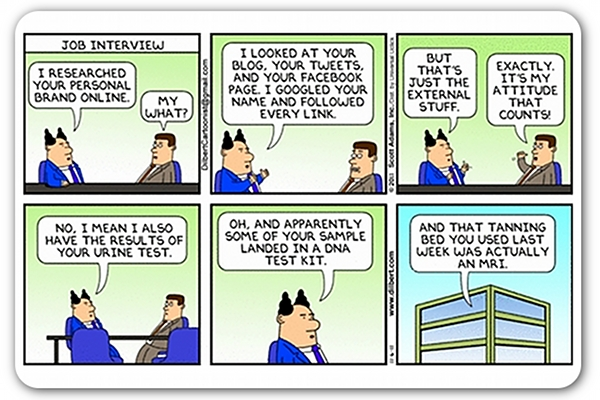
\includegraphics[scale=.5]{assets/personal-brand}
	\end{figure}
\end{frame}

%what

\begin{frame}
	\begin{figure}
		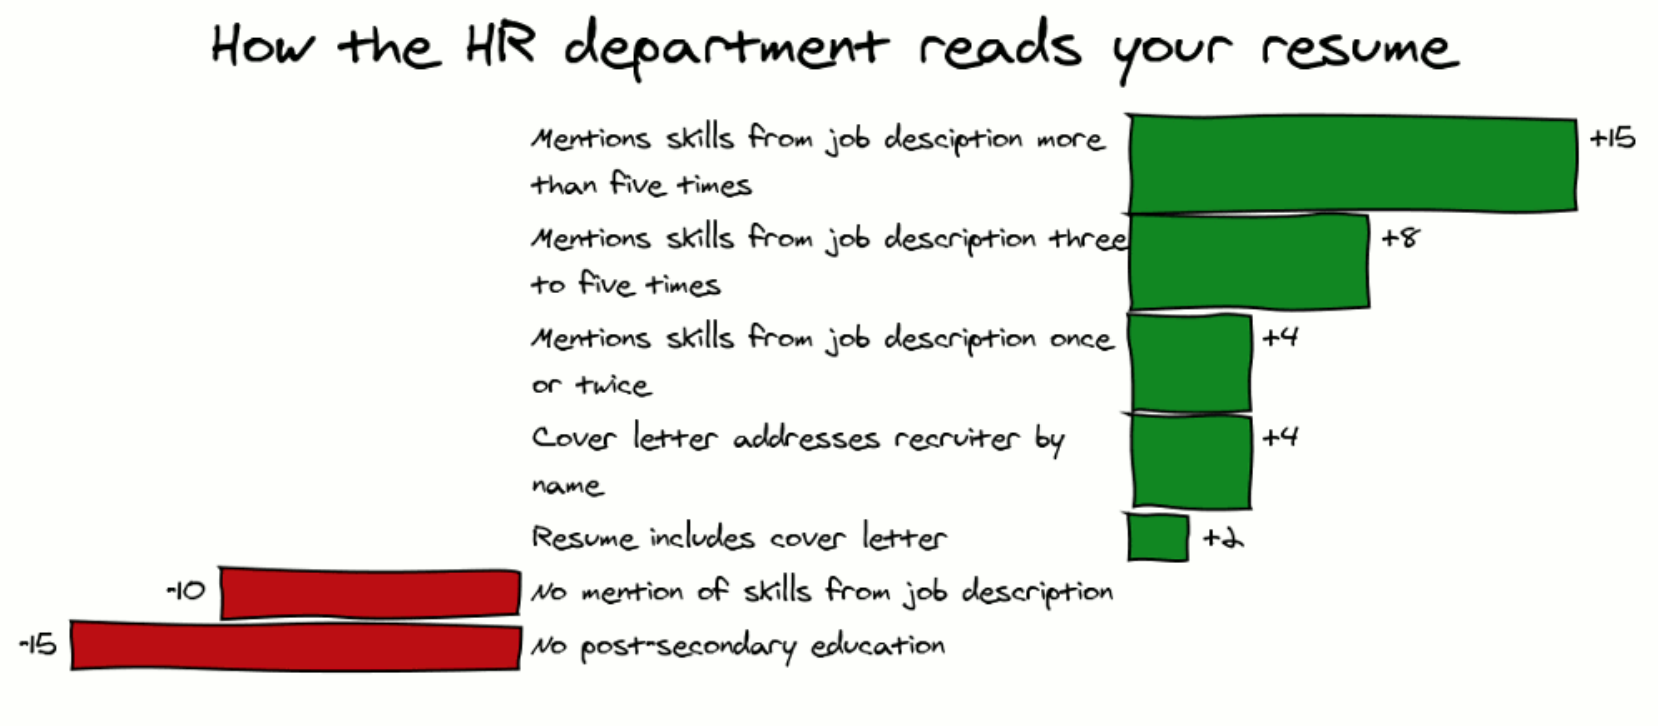
\includegraphics[scale=.35]{assets/diff1}
	\end{figure}
\end{frame}

\begin{frame}
	\begin{figure}
		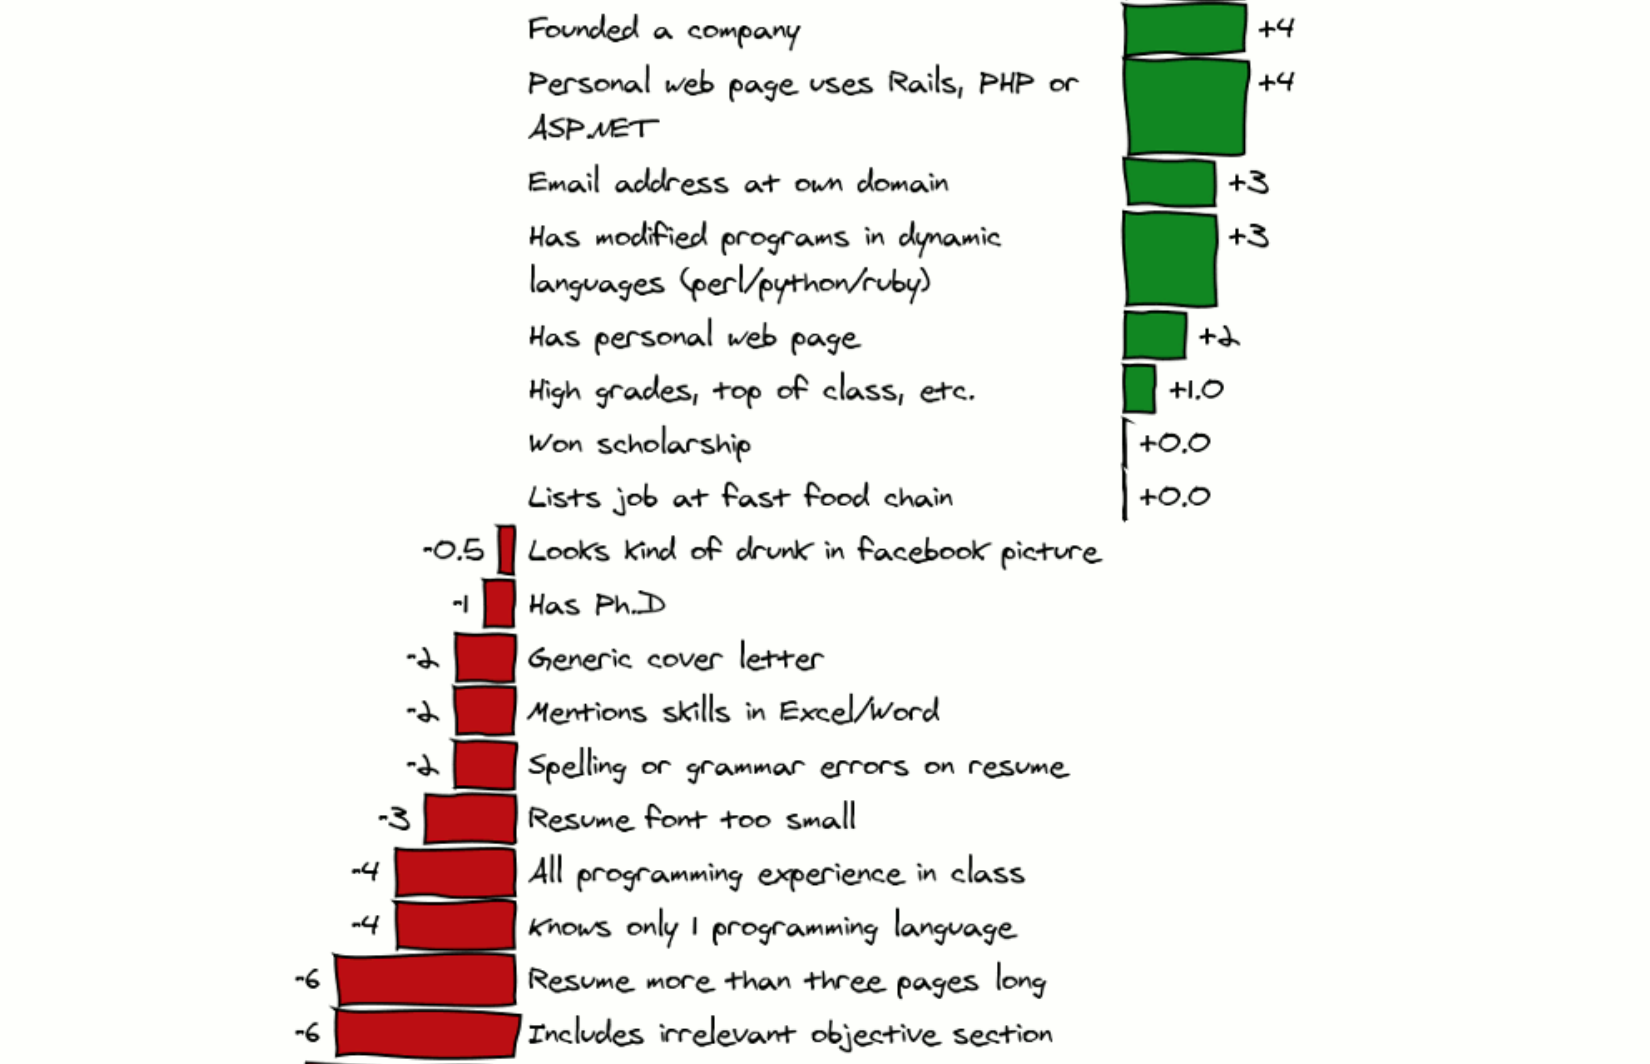
\includegraphics[scale=.35]{assets/diff2}
	\end{figure}
\end{frame}

\begin{frame}
	\begin{figure}
		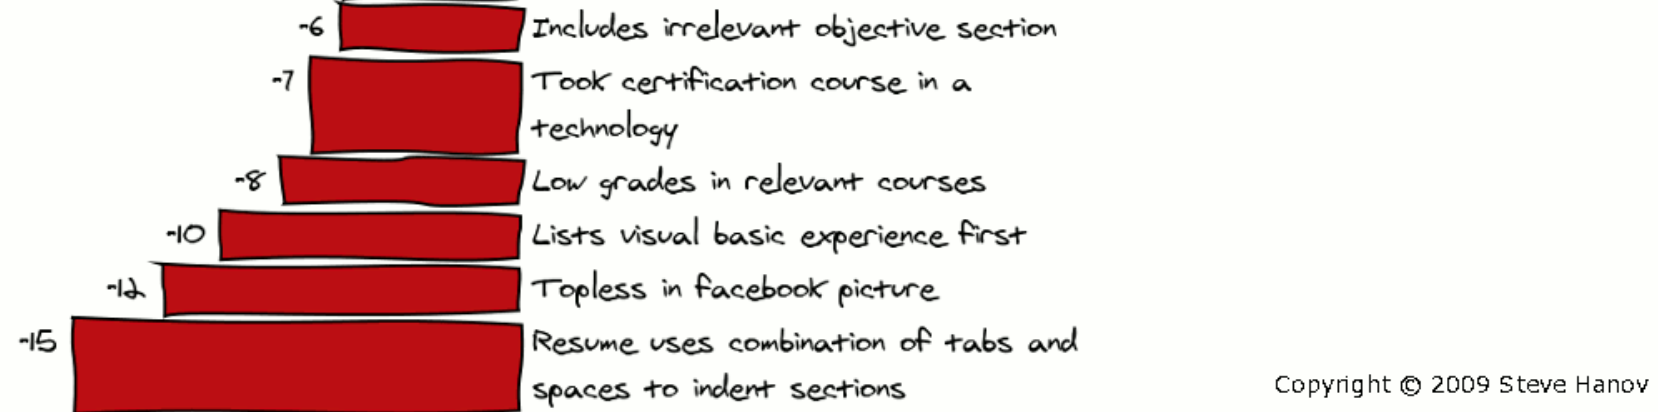
\includegraphics[scale=.35]{assets/diff3}
	\end{figure}
\end{frame}

\begin{frame}
	\begin{figure}
		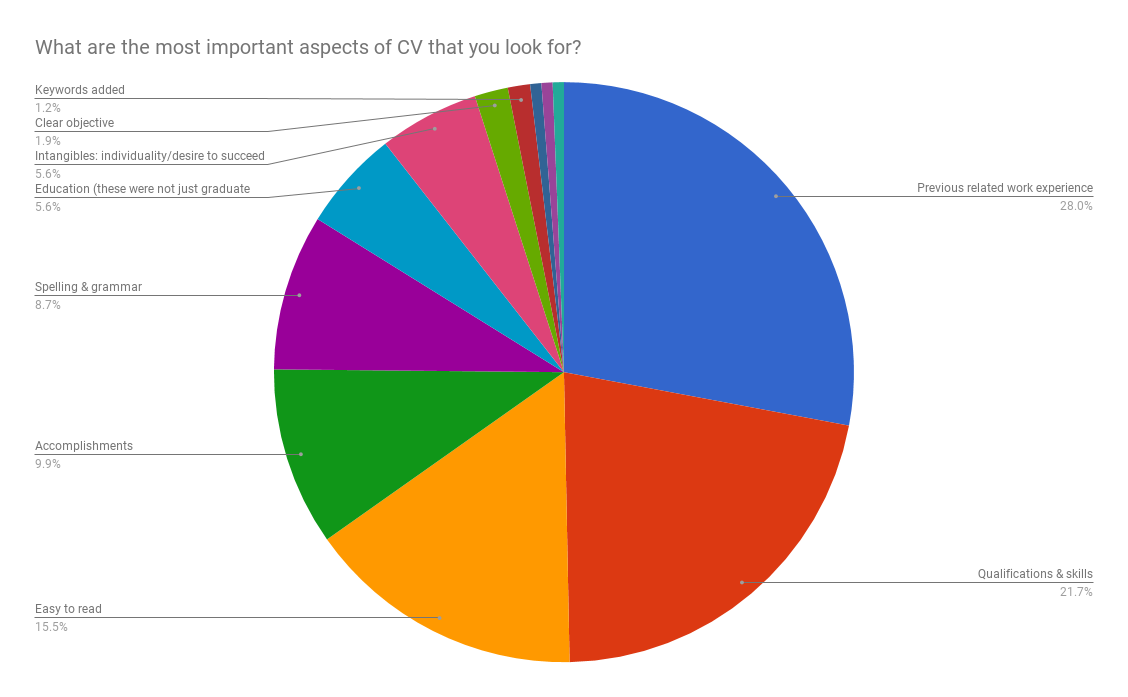
\includegraphics[scale=.27]{assets/priority}
		\caption{2010 Employers Survey}
	\end{figure}
	\href{http://stevehanov.ca/blog/resume_comic.png}{source}
\end{frame}

\begin{frame}
	\begin{figure}
		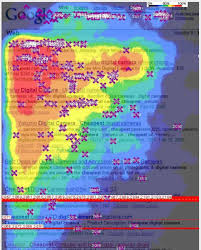
\includegraphics[scale=.8]{assets/golden-triangle}
		
	\end{figure}
	\href{www.forbes.com/sites/roberthof/2015/03/03/how-do-you-google-new-eye-tracking-study-reveals-huge-changes/\#604c90423828}{source}
\end{frame}

\begin{frame}
	\frametitle{No One Size Fits All}
	\begin{figure}
		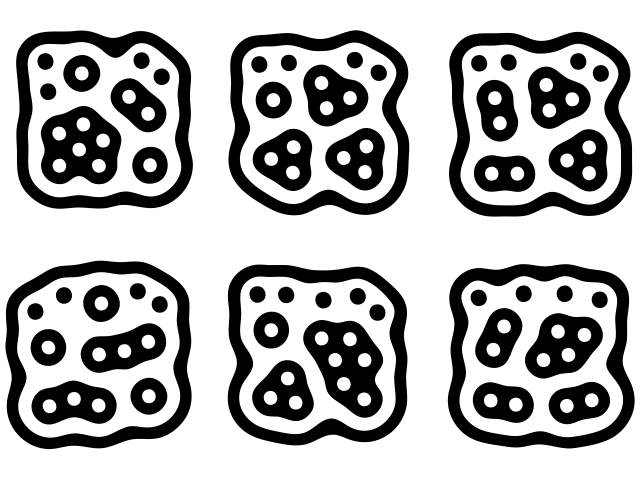
\includegraphics[scale=.5]{assets/reactivision}
	\end{figure}
\end{frame}



\begin{frame}
	\frametitle{When?}
	\pause fluid document
	\pause Grows with you
	\pause Becomes more tailored to you career 
	\pause More you! 
	
\end{frame}

%CONTENT

\begin{frame}
	\frametitle{Personal Details}
	
	\begin{itemize}
		\item Name (Obviously)
		\item Address
		\item Telephone Numbers
		\item Email
		\item Website Address (Portfolio)
	\end{itemize}

	\pause
	You are not required to provide any further information. 
	\begin{itemize}
		\item Age
		\item Gender
		\item Nationality
		\item ... 
	\end{itemize}

\end{frame}

\begin{frame}
	\frametitle{No Rockstar Profile Pic

\end{frame}

\begin{frame}
	\frametitle{DON'T}

	\begin{itemize}
		\item Lie. 
		\item Make it more than 3 pages. Remember less is more if you express it clearly. 2 pages is great, 1 page is ideal.
 		\item Include your age, a photo, jokey email addresses, your marital status or slang.
		\item Use more than two fonts or colours.
		\item Avoid bad grammar, spelling or too many long sentences. If you don't double check the basics in your CV, employers can?t trust that you'll check things at work.
		\item Repeat yourself. You only need to say it clearly once.
	\end{itemize}
\end{frame}


\end{document}
